\documentclass[dvipsnames]{article}

\usepackage[margin=0.5in]{geometry}
\usepackage{amsmath}
\usepackage{tikz}
\usepackage{pgfplots}

\usetikzlibrary{arrows.meta}

\begin{document}
	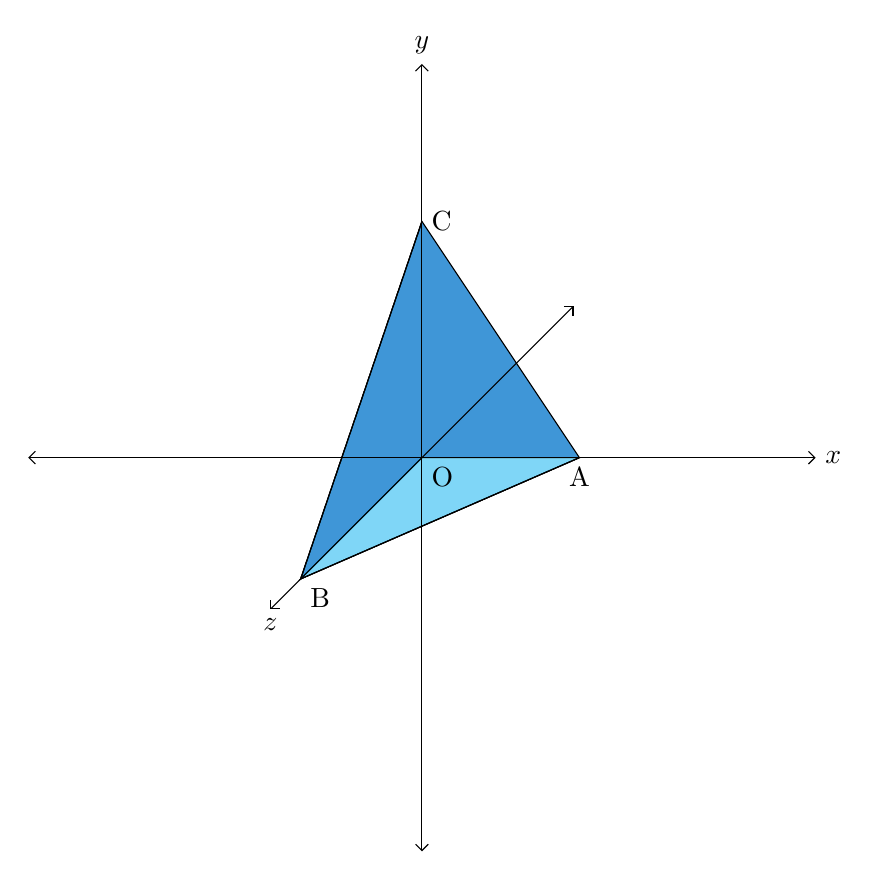
\begin{tikzpicture}
		\filldraw[fill=NavyBlue,fill opacity=0.5] (0,0,0) -- (0,0,4) -- (0,3,0);
		\filldraw[fill=White,fill opacity=0.5] (0,0,0) -- (0,0,4) -- (2,0,0);
		\filldraw[fill=NavyBlue,fill opacity=0.5] (2,0,0) -- (0,0,0) -- (0,3,0);
		\filldraw[fill=cyan,fill opacity=0.5] (2,0,0) -- (0,0,4) -- (0,3,0);
		
		\node[below right] (1) at (0,0,0) {$\text{O}$};
		\node[below] (2) at (2,0,0) {$\text{A}$};
		\node[below right] (3) at (0,0,4) {$\text{B}$};
		\node[right] (4) at (0,3,0) {$\text{C}$};
		
		\node[right] (x) at (5,0,0) {$x$};
		\node[above] (y) at (0,5,0) {$y$};
		\node[below] (z) at (0,0,5) {$z$};
		
		\draw[Straight Barb-Straight Barb] (5,0,0) -- (-5,0,0);
		\draw[Straight Barb-Straight Barb] (0,5,0) -- (0,-5,0);
		\draw[Straight Barb-Straight Barb] (0,0,5) -- (0,0,-5);
		
		\draw (0,0,0) -- (2,0,0) -- (0,0,4) -- (0,3,0) -- (2,00) -- cycle;
	\end{tikzpicture}
	\\\null\\
	Where \\ 
	\indent $\text{A}=(2,0,0)$ \\
	\indent $\text{B}=(0,0,4)$ \\
	\indent $\text{C}=(0,3,0)$ \\
	\indent $\text{O}=(0,0,0)$ \\
\end{document}